\chapter{Điều khiển và cải tiến tránh vật cản cho robot}}
%===================

\section{Đặt vấn đề}
%------------------

% Nhắc lại vấn đề ở phần cuối chương 1
Công nghệ SLAM là công nghệ cốt lõi trong robot tự hành thông minh, hiện nay công nghệ SLAM 2D chiếm phần lớn trong các ứng dụng do tính đơn giản, giá thành hợp lý. Tuy nhiên, với SLAM 2D, robot chỉ có thể tạo được bản đồ và di chuyển, tránh vật cản khi có thông tin về vật cản đó trên một mặt phẳng mà LIDAR quét được. Trong thực tế, môi trường hoạt động của chúng có nhiều loại vật thể có hình dạng, kích thước và chiều cao khác nhau.

Để giải quyết vấn đề này, có một số phương pháp như:
\begin{itemize}
    \item Thêm một số tầng cảm biến khác theo chiều cao thân robot như robot RHINO (\cite{Buhmann1995})
    \item Sử dụng cảm biến LIDAR 3D (\cite{Pierzchala2018})
    \item Ứng dụng visual-based SLAM (\cite{Chen2000, Mittal2019})
\end{itemize}

Các phương pháp trên có nhược điểm là chi phí thiết bị cao, chi phí tính toán lớn do robot phải xử lý lượng lớn dữ liệu đầu vào. Trong luận văn này , để đảm bảo robot có thể hoạt động được theo thời gian thực và tích hợp trên hệ thống sẵn có, tác giả sử dụng phương pháp tích hợp thêm một tầng cảm biến khoảng cách hồng ngoại để phối hợp với Lidar và cảm biến siêu âm có sẵn trên robot để hỗ trợ và tăng cường tránh vật cản cho robot. Tác giả thực hiện một số nhiệm vụ như sau:

\begin{itemize}
    \item Thiết kế mạch lấy dữ liệu cảm biến
    \item Lập trình lấy dữ liệu và xử lý dữ liệu từ các cảm biến khoảng cách hồng ngoại
    \item Đề xuất giải thuật điều khiển tránh vật cản bằng hệ thống cảm biến khoảng cách hồng ngoại.
    \item Phối hợp để phân quyền điều khiển robot
    \item Tích hợp tín hiệu từ cảm biến để cập  nhật dữ liệu vật cản vào bản đồ di chuyển của robot
    \item Đánh giá kết quả và hiệu quả của hệ thống
\end{itemize}

\section{Giới thiệu nền tảng robot}
\label{sec:RobotIntro}
% - Kiến trúc phần cứng của robot
% - Ứng dụng hệ điều hành ROS
% - Các bài toán điều khiển trên rb

Luận văn này được thực hiện trên nền tảng robot di động EAI Dashgo D1 \figurename{ \ref{fig:dashgoD1}} là một nền tảng robot di động thông minh được sản xuất phục vụ nghiên cứu về robot tự hành và Hình \ref{fig:airhustbot} là robot đang trong quá trình phát triển thành robot dịch vụ thông minh.

% \subsection{Phần cứng}

% \begin{figure}[htp]
% 	\centering
% 	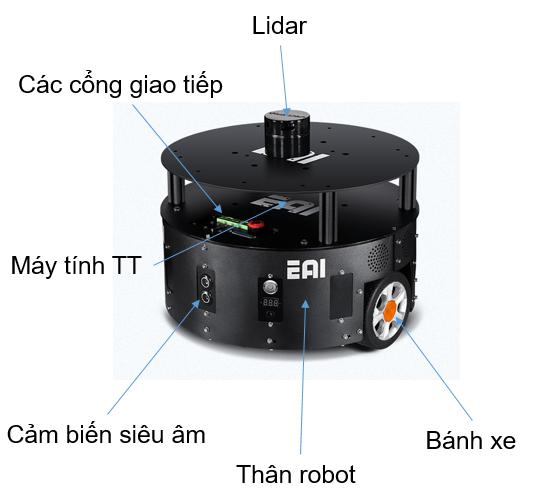
\includegraphics[width=0.7\linewidth]{figures/dashgoD1.JPG}
% 	\caption{Nền tảng robot di động Dashgo D1}
% 	\label{fig:dashgoD1}
% \end{figure}

\begin{figure}[htbp]
    \centering
    \subfloat[][]{
        \label{fig:dashgoD1}
        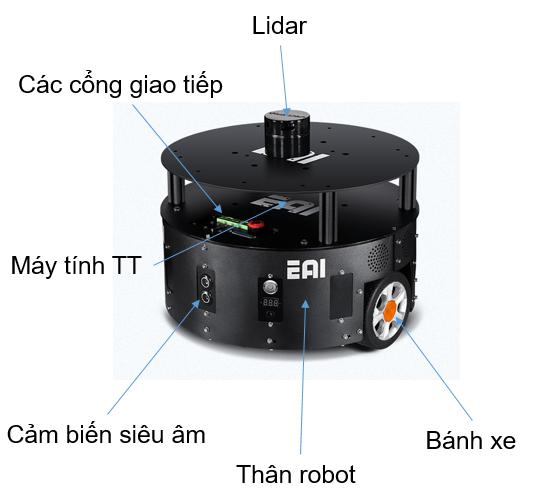
\includegraphics[width=0.5\linewidth]{figures/dashgoD1.JPG}}
    \subfloat[][]{
        \label{fig:airhustbot}
        \includegraphics[width=0.4\linewidth]{figures/airhustbot.png}}
    \caption{Nền tảng robot di động}
    \label{fig:platformRobto}
\end{figure}

Robot có cấu tạo gồm 3 phần chính: Phần chân đế thực hiện chức năng di chuyển, phần cảm biến và phần điều khiển trung tâm.

\begin{figure}[htbp]
	\centering
	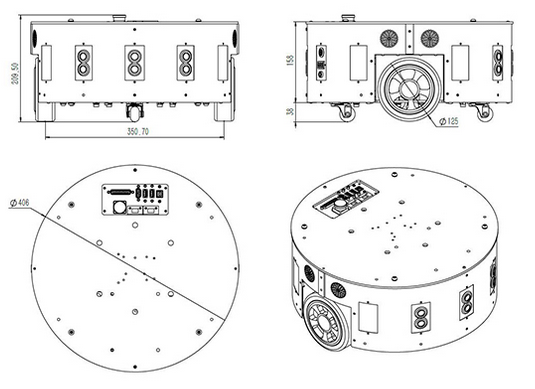
\includegraphics[width=0.7\linewidth]{figures/dashgo_base.png}
	\caption{Cấu tạo phần chân đế}
	\label{fig:dashgoBase}
\end{figure}

\subsection{Phần chân đế}
Phần chân đế có cấu tạo gồm hai bánh chủ động và 2 bánh xe bị động (\figurename{ \ref{fig:dashgoBase}}). Động cơ có gắn encoder độ chính xác cao để phản hồi vị trí. Phần chân đế được điều khiển bởi mạch điều khiển được mở rộng từ mạch arduino kết hợp với các module điều khiển bánh xe. Hoạt động của robot nhờ nguồn điện 12V từ acquy với thời gian sạc đầy khoảng 4 tiếng.

\subsection{Phần cảm biến}
Robot được trang bị bốn cảm biến siêu âm và một cảm biến LIDAR. Bốn cảm biến siêu âm sử dụng cho mục đích tránh vật cản. Nguyên lý hoạt động của cảm biến siêu âm như sau:
\begin{itemize}
    \item Đầu phát của cảm biến phát ra sóng siêu âm
    \item Sóng siêu âm bị dội lại khi có vật cản
    \item Thực hiện đo khoảng cách từ lúc phát tới lúc nhận được sóng dội lại, tính toán dựa trên tốc độ di chuyển sóng âm trong không khí ta tính được khoảng cách từ cảm biến tới vật.
\end{itemize}
Cảm biến siêu âm có các ưu điểm như không bị ảnh hưởng bởi màu sắc của vật, hoạt động tốt trong môi trường tối, tiêu tốn ít năng lượng và dễ dàng kết nối với các vi điều khiển. Tuy nhiên nó cũng có các điểm hạn chế như giới hạn khoảng cách đo được, độ phân giải và tần số đo thấp do đó nó không phù hợp với các ứng dụng có vật đích di chuyển nhanh. Cảm biến siêu âm không hoạt động được với các bề mặt không bằng phẳng, các bề mặt hấp thụ âm thanh.

Cảm biến YDLIDAR G4 sử dụng tia laser sử dụng đạt tiêu chuẩn an toàn FDA Class 1 \footnote{Tiêu chuẩn Laser FDA Class 1: Được xem là không gây nguy hiểm. Mức độ nguy hiểm tăng khi nhìn qua kính hội tụ quang học như kính lúp, kính hiển vi. Theo \url{www.fda.gov}}.
Cảm biến tích hợp một động cơ để quay quét mắt laser ${360}^{o}$ với tần số quét từ 5-12Hz. Đo khoảng cách bằng laser với giải đo từ 0.10 - 16m với tần số lấy mẫu có thể đạt 9000Hz.
Cảm biến này được sử dụng cho việc tạo bản đồ, điều hướng và tránh vật cản.


\subsection{Hệ thống phần mềm}
%       - Cấu trúc phần mềm: Linux-> ROS-> Package -> Subpackage
%       - Quy trình thực hiện một ứng dụng di chuyển tới các vị trí xác định trong văn phòng: Tạo bản đồ: gmapping -> Di chuyển trong bản đồ, dùng rviz (giống Hand-on)

\begin{figure}[htbp]
    \centering
    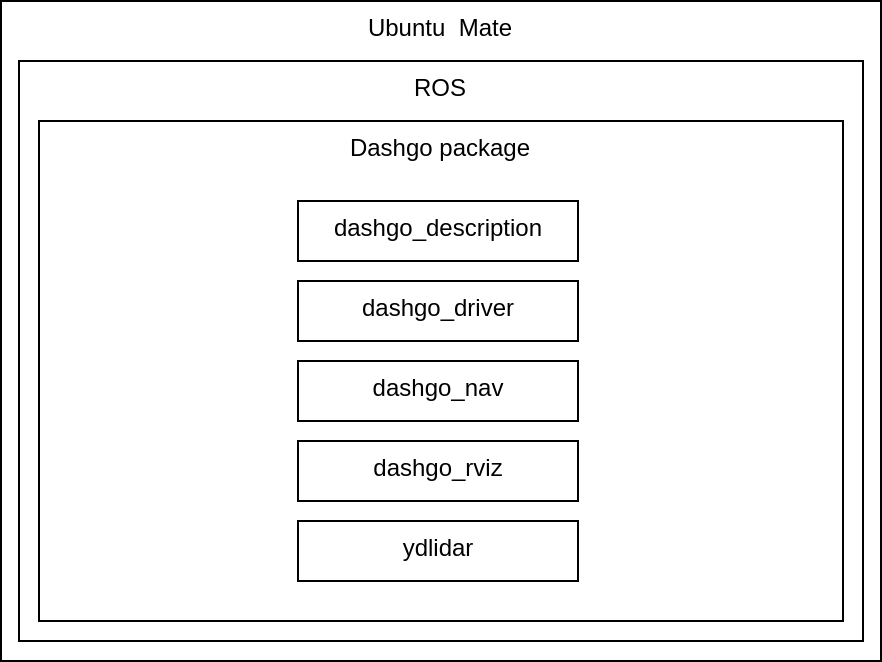
\includegraphics[width=0.7\linewidth]{figures/dashgo-architecture.png}
    \caption{Kiến trúc phần mềm điều khiển robot trên Dashgo D1}
    \label{fig:dashgo-architecture}
\end{figure}

Robot sử dụng mạch Raspberry Pi 3 làm bộ điều khiển trung tâm. Chạy hệ điều hành robot ROS Kinetic trên nền tảng Ubuntu MATE 16.04. Để thực hiện các chức năng cơ bản như định vị, tạo bản đồ, di chuyển tới vị trí xác định trong bản đồ, tránh vật cản trong quá trình di chuyển, robot cần phải được cài đặt gói chương trình dashgo được cung cấp bởi nhà sản xuất.
\figurename{ \ref{fig:dashgo-architecture}} mô tả kiến trúc phần mềm trên Dashgo D1. Trong đó:
\begin{itemize}
    \item \codeword{dashgo_description} là gói chứa các mô tả của robot, được dùng trong hiển thị Rviz và mô phỏng robot trong Gazebo.
    \item \codeword{dashgo_driver} chứa các thông số cấu hình và chương trình driver để điều khiển robot.
    \item \codeword{dashgo_nav} chứa các chương trình điều khiển robot, bao gồm \codeword{gmapping} để tạo bản đồ môi trường và \codeword{navigation} để thực hiện di chuyển tự động trong bản đồ.
    \item \codeword{dashgo_rviz} chứa các file mẫu rviz của một số tác vụ cơ bản.
    \item \codeword{dashgo_tools} chứa các công cụ để làm việc với robot.
    \item \codeword{ydlidar} là gói quản lý, driver của YDLIDAR.
\end{itemize}

\section{Điều khiển Dashgo robot}
%TODO:
% <<\textit{1. Các bước thực hiện tạo bản đồ, lưu bản đồ bằng gmapping -> Navigation: ước tính vị trí, di chuyển tới các điểm xác định trong bản đồ\\}
% \textit{2.Đánh giá hoạt động của robot}>>

Dashgo D1 ứng dụng giải thuật SLAM và hoạt động trên nền tảng hệ điều hành ROS.
Hai chức năng chính là tạo bản đồ môi trường mới và điều hướng trong môi trường đã biết.

\subsection{Quy trình thực hiện}

\textbf{Tạo bản đồ:} Với một môi trường chưa biết trước, việc đầu tiên là phải tạo bản đồ.
Chương trình tạo bản đồ được tạo sẵn trong file \codeword{gmapping.launch}

\begin{lstlisting}
$ roslaunch dashgo_nav gmapping.launch
\end{lstlisting}

Chương chương trình này sẽ gọi tới một số chức năng khác như driver điều khiển chân đế \codeword{driver.launch}, driver lidar \codeword{lidar.launch}, chạy thuật toán và khai báo các thông số tại \codeword{gmapping_base.launch}

Sau khi chạy file \codeword{gmapping.launch}, bật Rviz lên để xem vị trí của robot và bản đồ.
\begin{lstlisting}
$ roslaunch dashgo_rviz view_navigation.launch
\end{lstlisting}
%TODO: đặt hình ảnh rviz vào đây.


Sử dụng công cụ di chuyển robot bằng tay để thu thập thông tin tạo bản đồ của môi trường. Chúng ta có thể sử dụng bàn phím hoặc app để di chuyển robot. Cho robot di chuyển trong toàn bộ môi trường để thực hiện thu thập thông tin cho bản đồ. Theo dõi trực quan trên Rviz để quan sát bản đồ tạo được.
\begin{lstlisting}
$ rosrun dashgo_tools teleop_keyboard.py
\end{lstlisting}

Sau đó lưu bản đồ lại bằng lệnh:
\begin{lstlisting}
$ cd dashgo_nav/maps
$ rosrun map_server map_saver -f <Ten ban do>
\end{lstlisting}

\textbf{Điều hướng:} Chương trình này sử dụng bản đồ đã được lưu, sử dụng thuật toán amcl để định vị và điều hướng trong bản đồ đã biết.
\begin{lstlisting}
$ roslaunch dashgo_nav navigation.launch
\end{lstlisting}

Bật Rviz:
\begin{lstlisting}
$ roslaunch dashgo_nav navigation.launch
\end{lstlisting}
%TODO: Thêm hình ảnh rviz lúc di chuyển
Trên giao diện Rviz, chúng ta sử dụng công cụ \codeword{2D Pose Estimate} để định vị lại vị trí của robot trong bản đồ bằng tay.
Bởi vì khi mới khởi tạo, robot chưa có đủ thông tin để tự định vị nó đang ở đâu trong bản đồ. Bước định vị bằng tay này không cần quá chính xác bởi vì sau khi robot di chuyển nó sẽ tự mình định vị và điều chỉnh vị trí của robot trong bản đồ. Sau đó, để điều hướng robot đến một điểm bất kì, chúng ta sử dụng công cụ \codeword{2D Nav Goal}. Ngoài ra, trên giao diện Rviz chúng ta còn có thể thấy các thông tin về: vị trí của robot, bản đồ, costmap\dots

\begin{figure}[htbp]
    \centering
    \subfloat[]{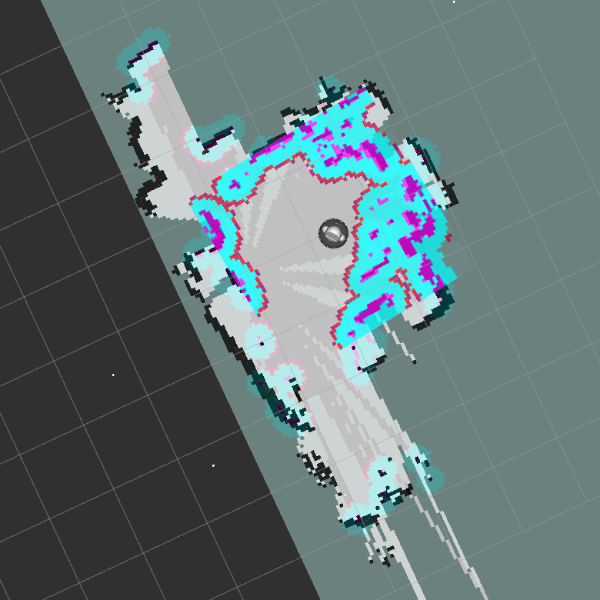
\includegraphics[width=0.45\linewidth]{figures/RB_mapping.png}}
    \subfloat[]{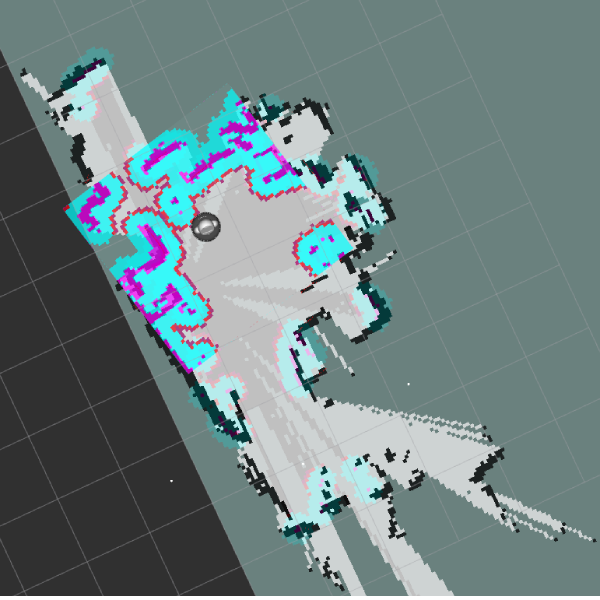
\includegraphics[width=0.45\linewidth]{figures/RB_mapping02.png}}
    \caption{Robot đang tạo bảo đồ thể hiện trên Rviz}
    \label{fig:mapping}
\end{figure}

\begin{figure}[htbp]
    \centering
    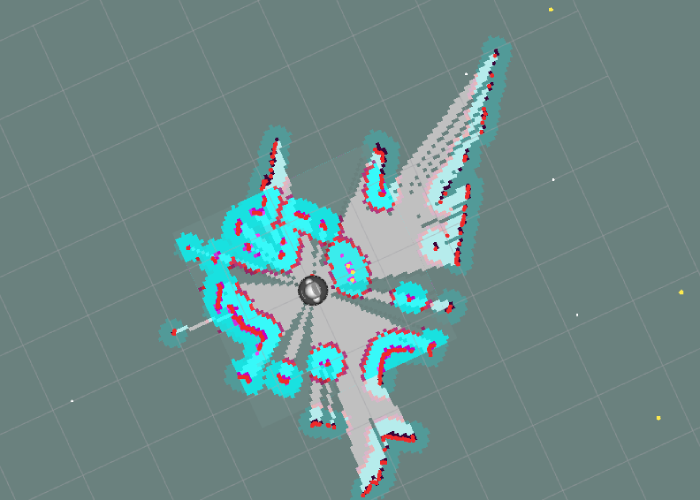
\includegraphics[width=0.6\linewidth]{figures/RB_navigation.png}
    \caption{Robot di chuyển tới đích trong bản đồ}
    \label{fig:navigation}
\end{figure}

Hình \ref{fig:mapping} thể hiện quá trình tạo bản đồ của robot.
Hình \ref{fig:navigation} thể hiện robot đang di chuyển tới vị trí đích xác định trong bản đồ. Đường màu xanh lá là đường đi dự kiến được tính toán dựa trên bản đồ giá trị (costmap).

\subsection{Đánh giá hoạt động của robot}
%FIXME: Đánh giá thêm
% Trong luận văn này, tác giả thực hiện 2 nhiệm vụ chính: Làm chủ điều khiển robot di động và cải tiến tránh vật cản bằng cảm biến khoảng cách hồng ngoại.

Với nền tảng robot hiện tại, hệ thống robot thực hiện được một số chức năng như sau:

\begin{itemize}
    \item Tạo bản đồ môi trường mới
    \item Di chuyển trong môi trường đã biết, điều hướng tới đích được cho.
    \item Tránh vật cản trong quá trình di chuyển.
\end{itemize}

Tuy nhiên bên cạnh đó cũng có một số hạn chế như sau:

\begin{itemize}
    \item Robot chỉ phát hiện và tránh vật cản được ở hai tầng cảm biến hiện tại (tương ứng với mặt phẳng đi qua cảm biến siêu âm và mặt phẳng quét của cảm biến LIDAR). Khi đó robot sẽ có một số hạn chế khi di chuyển trong môi trường có các vật có hình dạng khác nhau như bàn, ghế xoay\dots
    \item Cảm biến siêu âm tránh vật cản không phát hiện được vật cản có bề mặt hấp thụ sóng âm thanh
    \item Cảm biến laser sử dụng cho nhiệm vụ định vị, điều hướng và cả tránh vật cản, vì vậy chi phí tính toán cao và thường phản ứng chậm với vật cản động.
\end{itemize}


\section{Cải tiến hệ thống tránh vật cản cho robot}
\label{sec:caitienhethongtranhvatcan}
% - Lắp thêm cảm biến và xử lý dữ liệu cảm biến
% - Trình bày giải thuật đề xuất
% - Áp dụng giải thuật phát hiện và tránh vật cản
% - Phối hợp các tầng cảm biến và phân quyền điều khiển robot

% \subsection{Đặt vấn đề}

Từ các hạn chế của robot hiện tại và với mục tiêu robot hoạt động hiệu quả trong môi trường biến động, tác giả đề xuất phương án bổ sung thêm một tầng cảm biến để phát hiện và tránh vật cản. Hệ thống này sử dụng một số cảm biến khoảng cách hồng ngoại, chi phí thiết bị và chi tính toán thấp để dễ dàng tích hợp được vào robot, phối hợp cùng với hai tầng cảm biến có sẵn nhưng vẫn đảm bảo robot hoạt động ổn định theo thời gian thực. Robot có thể phát hiện và tránh được đa dạng vật cản hơn. Dựa trên các kết quả tham khảo ở \ref{sec:tranhVatCan_ref} tác giả đề xuất một mô hình giải thuật mới.

\subsection{Phần cứng}

% \begin{figure}[htbp]
    %     \centering
    %     \subfloat[][]{
        %         \label{fig:arduino}
        %         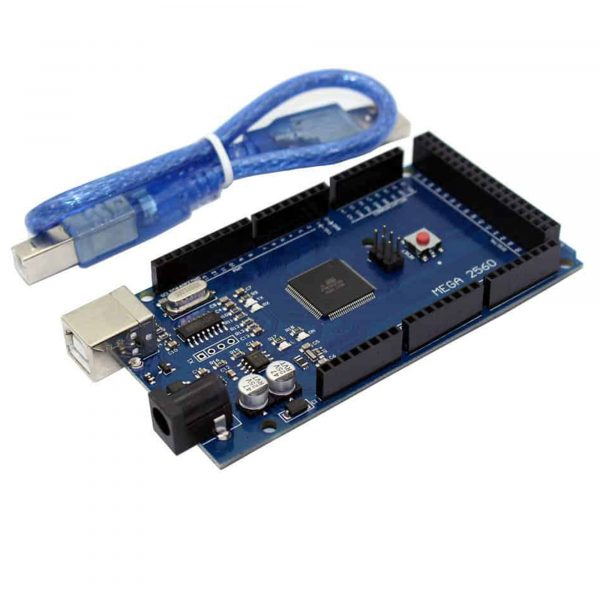
\includegraphics[width=0.5\linewidth]{figures/arduinoMega.jpg}}
        %     \subfloat[][]{
            %         \label{fig:irSharp}h
%         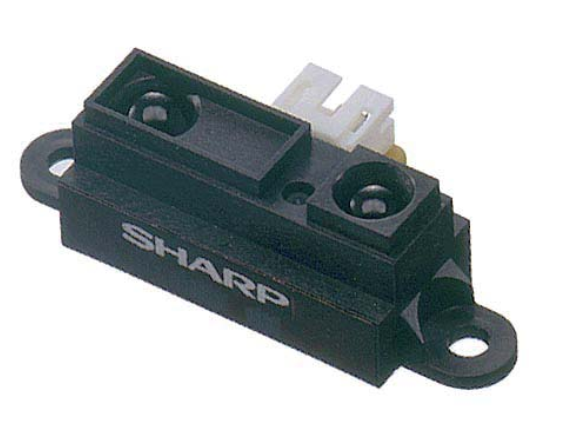
\includegraphics[width=0.4\linewidth]{figures/IRsharp.png}}
%     \caption{Phần cứng sử dụng}
%     \label{fig:components}
% \end{figure}

Hệ thống gồm một số cảm biến hồng ngoại IR Sharp GP2Y0A21YK0F và mạch Arduino Mega 2560. Vị trí các cảm biến được bố trí như \figurename{ \ref{fig:IR_layout}}.

\begin{figure}[htbp]
	\centering
	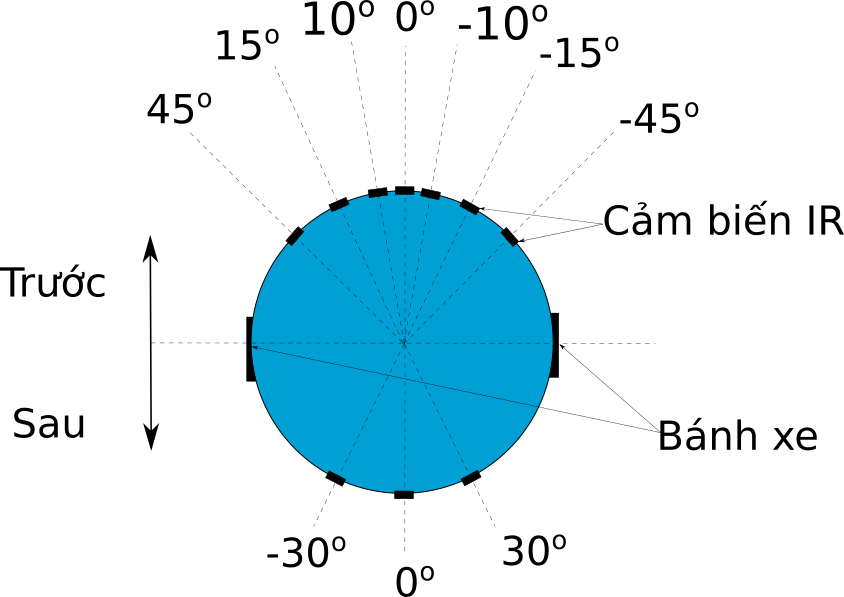
\includegraphics[width=0.7\linewidth]{figures/IR_layout.png}
	\caption{Sơ đồ bố trí cảm biến}
	\label{fig:IR_layout}
\end{figure}

\begin{figure}[htbp]
    \centering
    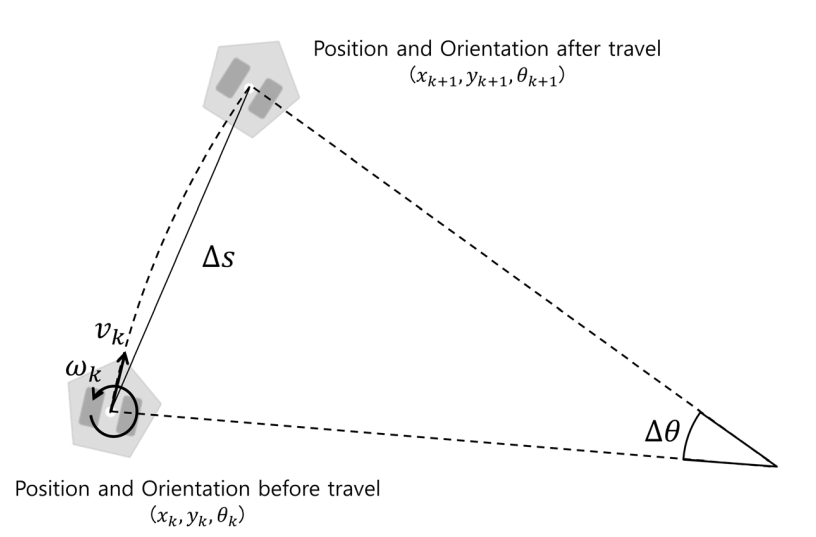
\includegraphics[width=0.7\linewidth]{figures/dead-reckoning.png}
    \caption{Dead reckoning \cite{pyo2017ros}}
    \label{fig:dead-reckoning}
\end{figure}

Trong quá trình di chuyển, robot có thể tiến và lùi vì vậy cần phải đặt cảm biến ở cả trước và phía sau robot.
Robot sử dụng hai bánh dẫn động chính và di chuyển trên mặt phẳng, do vậy chuyển động của robot được quy về hai thông số vận tốc dài $v$ và vận tốc góc $\omega$ theo phương pháp ước tính trạng thái robot dead-reckoning Hình \ref{fig:dead-reckoning} \cite{pyo2017ros}.
Do đó tác giả đề xuất phương án mới đặt cảm biến dày hơn ở khu vực chính giữa và thưa ra hai bên như \figurename{ \ref{fig:IR_layout}}.

\subsection{Xử lý dữ liệu cảm biến}

\begin{figure}[htbp]
    \centering
    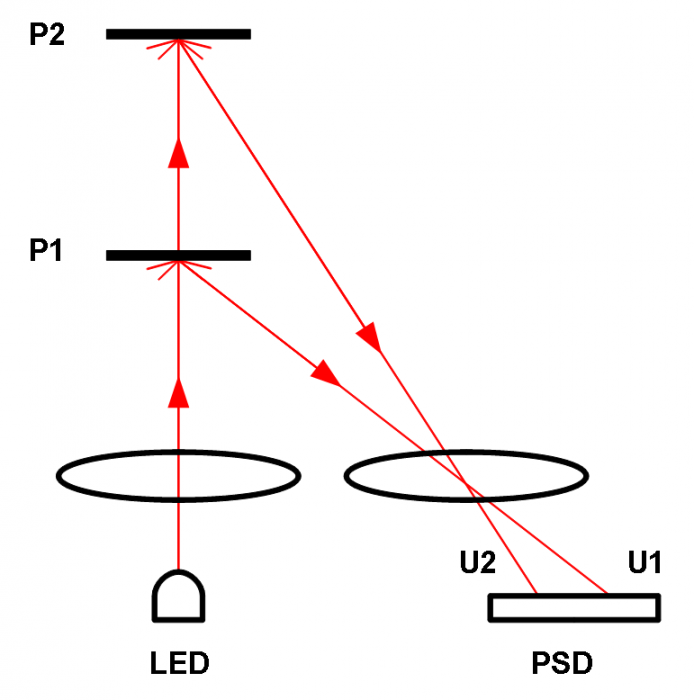
\includegraphics[width=0.5\linewidth]{figures/sensor_ir_distance_principle.png}
    \caption{Cơ chế hoạt động của cảm biến khoảng cách hồng ngoại}
    \label{fig:sensor_ir_distance_principle}
\end{figure}

\begin{figure}[htbp]
    \centering
    \subfloat[][]{
        \label{fig:irSharp-vol-distance}
        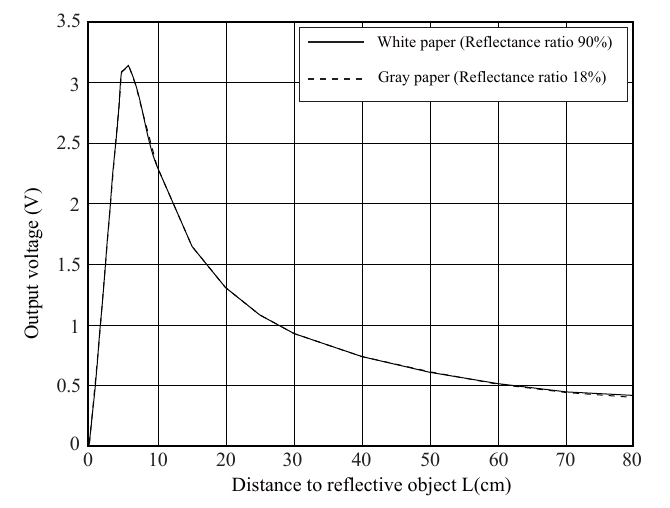
\includegraphics[width=0.5\linewidth]{figures/irSharp-vol-distance.png}
    }
    \subfloat[][]{
        \label{fig:irSharp-vol-distance_2}
        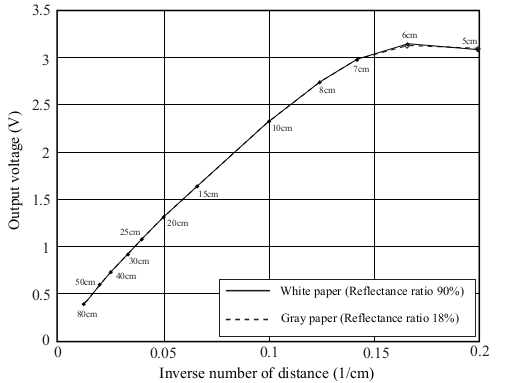
\includegraphics[width=0.5\linewidth]{figures/irSharp-vol-distance_2.png}
    }
    \caption{Mối liên hệ giữa khoảng cách và điện áp}
    \label{fig:irSharp-vol-distance}
\end{figure}

Cảm biến khoảng cách hồng ngoại là loại cảm biến sử dụng ánh sáng hồng ngoại với một đầu phát và một đầu thu. Cơ chế hoạt động của cảm biến khoảng cách hồng ngoại như \figurename{ \ref{fig:sensor_ir_distance_principle}}. Trong đó, đề LED phát tia sáng hồng ngoại, khi gặp vật cản, tia sáng sẽ bị phản xạ lại, in lên tấm PSD tại các vị trí tương ứng với góc chiếu khác nhau, tạo điện áp khác nhau từ U1 đến U2 \footnote{\url{https://home.roboticlab.eu/en/examples/sensor/ir_distance}}.

Mối quan hệ giữa điện áp ra và khoảng cách của module cảm biến khoảng cách hồng ngoại IR Sharp GP2Y0A21YK0F như \figurename{ \ref{fig:irSharp-vol-distance}} \footnote{\url{www.sparkfun.com/datasheets/Components/GP2Y0A21YK.pdf}}

\begin{figure}[htbp]
    \centering
    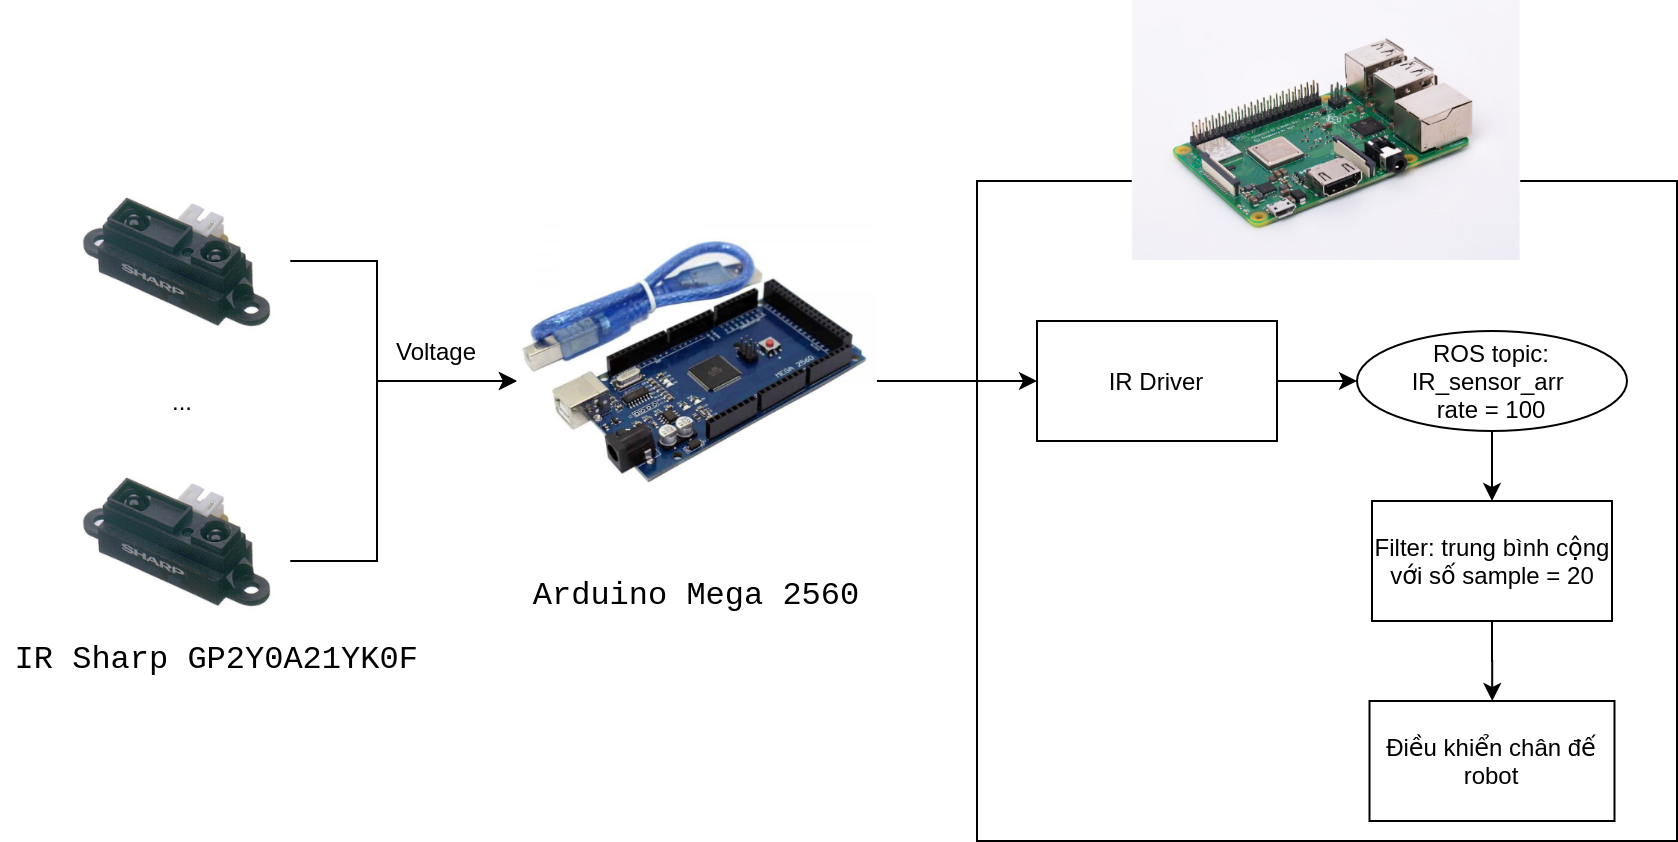
\includegraphics[width=\linewidth]{figures/ir_safety_controller-dataProcessing.png}
    \caption{sơ đồ xử lý dữ liệu cảm biến}
    \label{fig:workflow-dataProcessing}
\end{figure}

Mạch Arduino Mega sẽ đọc tín hiệu điện trả về từ các cảm biến IR mỗi khi có lệnh yêu cầu từ Raspberry Pi. Mỗi chân dữ liệu của cảm biến kết nối với chân Analog input trên mạch Arduino để đọc dữ liệu điện áp thông qua ADC 8 bit.
Trên Raspberry Pi, {\tt node ir\_driver} sẽ nhận các dữ liệu ADC của các cảm biến từ Arduino. \figurename{ \ref{fig:irSharp-vol-distance}} cho ta mối liên hệ giữa điện áp và khoảng cách của cảm biến SHARP GP2Y0A21YK0F. Tuy nhiên, đây là đồ thị một đường cong không được biểu diễn bởi một hàm toán học cụ thể. Phương pháp được sử dụng là dùng thí nghiệm đo với giá trị điện áp và khoảng cách tương ứng. Sau đó nội suy kết quả thí nghiệm thành một hàm toán học gần đúng. Trong luận văn này, sử dụng công thức \ref{equa:ADC2Vol} và \ref{equa:Vol2Distance} \footnote{\url{https://github.com/guillaume-rico/SharpIR}} và kiểm nghiệm thấy kết quả khá chính xác (tại \ref{sub:DanhgiaCBIR})

\begin{equation}
    v = \frac{ADC * 5.0}{1023.0}
    \label{equa:ADC2Vol}
\end{equation}

\begin{equation}
    d = 27.728 * {v}^{-1.2045}
    \label{equa:Vol2Distance}
\end{equation}

Trong đó:
\begin{itemize}
    \item v - Điện áp ghi nhận tại chân analog của arduino.
    \item d - Khoảng cách đo được từ cảm biến
\end{itemize}

Sau khi tính được khoảng cách của các cảm biến sẽ {\tt publish} ra {\tt topic IR\_sensor\_arr} chứa thông tin đo được từ tất cả các cảm biến với tần số 20Hz.
%FIXME: Hiện tại trong chương trình đang để tần số 100Hz, tuy nhiên xem lại data sheet thì tần số đo của cảm biến này chỉ đạt 26Hz.

\begin{equation}
    d = \frac{\sum_{i=1}^{N} d_i}{N}
    \label{equa:Med_filter}
\end{equation}

Sau đó dùng bộ lọc trung bình cộng để lấy trung bình cộng \ref{equa:Med_filter} của N lần đo để giảm tác động của nhiễu. Để đảm bảo hệ thống vừa hoạt động được theo thời gian thực và vừa đảm bảo độ chính xác, tin cậy, tác giả chọn N = 10 với tần số cập nhật 2 lần/giây (Chi tiết tại mục \ref{sub:DanhgiaCBIR})

\subsection{Trình bày giải thuật}
%TODO: Trình bày giải thuật điều khiển 2 mức: bubble boudary bên ngoài và vòng tròn nguy cấp bên trong. Tuy nhiên phần này chưa điều chỉnh thông số thuật toán nên

\begin{figure}[htbp]
    \centering
    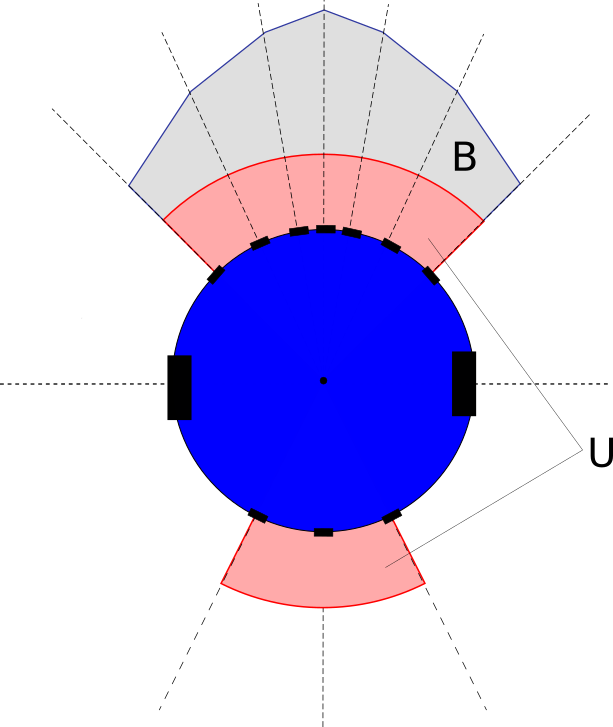
\includegraphics[width=0.5\linewidth]{figures/arg_obstacle-detection-area.png}
    \caption{Vùng xác định vật cản}
    \label{fig:arg-obstacle-area}
\end{figure}

Tác giả đề xuất sử dụng hai giải thuật để điều khiển robot tránh vật cản sử dụng tầng cảm biến hồng ngoại. Định nghĩa hai vùng phát hiện vật cản. Vùng B và vùng U như \figurename{ \ref{fig:arg-obstacle-area}}. Chúng ta đặt mức độ ưu tiên khác nhau cho từng vùng. Đặt cờ C1, C2 lần lượt thể hiện thuật toán phản ứng ở vùng B và vùng U.

\textbf{Vùng khẩn cấp U}:
Vùng này thể hiện vùng nguy hiểm, được xác định bằng một đường tròn bán kính ${R}_{U}$ từ tâm của robot. Khi phát hiện có vật cản nằm trong vùng này nếu robot có lệnh di chuyển tiến hoặc lùi thì sẽ dừng lại, di chuyển robot lùi/tiến để tránh khỏi vật cản, đồng thời phát âm thanh để thông báo có vật cản cho đến khi không còn vật cản trong vùng này.
\begin{figure}[]
    \centering
    \begin{tikzpicture}[node distance=2cm]
        % \node (start) [startstop] {Bắt đầu};
        \node (in1) [io] {Lấy dữ liệu cảm biến ${IR}_{i}$};
        \node (dec1) [decision, below of=in1] {${IR}_{i} < {R}_{U}$};
        \node (dec2) [decision, below of=dec1, aspect=2, node distance=4cm, xshift = -3cm] {$i = [0..7]$ và $v > 0$};
        \node (dec3) [decision, below of=dec1, aspect=2, node distance=4cm, xshift = 3cm] {$i = [8..10]$ và $v < 0$};
        % \node (dec4) [decision,text width=3.5cm, aspect=1.5, below of=dec1, node distance=3cm, xshift=5.5cm] {$i = [8..10]$ và $i = [0..7]$ và $v \neq 0$};
        \node (proc1) [process, below of=dec2, node distance=3cm,xshift = 0cm] {Lùi + Phát âm thanh};
        \node (proc2) [process, below of=dec3, node distance=3cm,xshift = 0cm] {Tiến + Phát âm thanh};

        % \draw [arrow] (start) -- (in1);
        \draw [arrow] (in1) --  (dec1);
        \draw [arrow] (dec1) -- (0,-3.5) -| (dec2);
        \draw [arrow] (dec2) -- node[anchor=east] {Đúng}(proc1);
        \draw [arrow] (dec2) --++ (-3,0) |- node[anchor=east] {Sai} (in1);
        \draw [arrow] (dec3) -- node[anchor=east] {Đúng}(proc2);
        \draw [arrow] (dec3) --++ (3,0) |- node[anchor=west] {Sai} (in1);
        % \draw [arrow] (dec2) -- node[anchor=east] {Sai}(dec3);
        \draw [arrow] (dec1) -- node[anchor=east] {Đúng}(0,-3.5) -| (dec3);
    \end{tikzpicture}
    \caption{Sơ đồ giải thuật vùng khẩn cấp U}
    \label{flowchart-urgent}
\end{figure}

\begin{figure}[htbp]
    \centering
    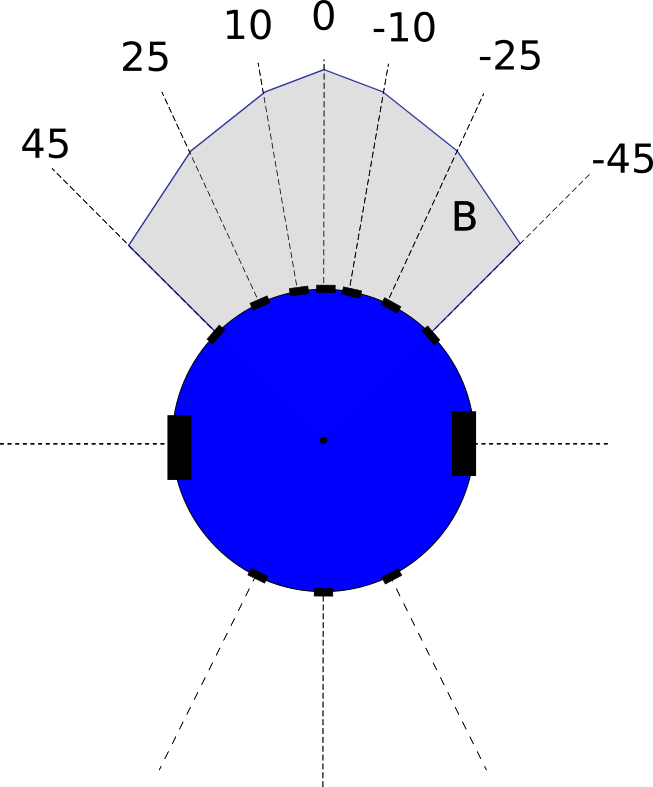
\includegraphics[width=0.4\linewidth]{figures/BB-argorithm.png}
    \caption{Hình dạng bong bóng phản ứng}
    \label{fig:BB-argorithm}
\end{figure}

\begin{figure}[htbp]
    \centering
    \subfloat[]{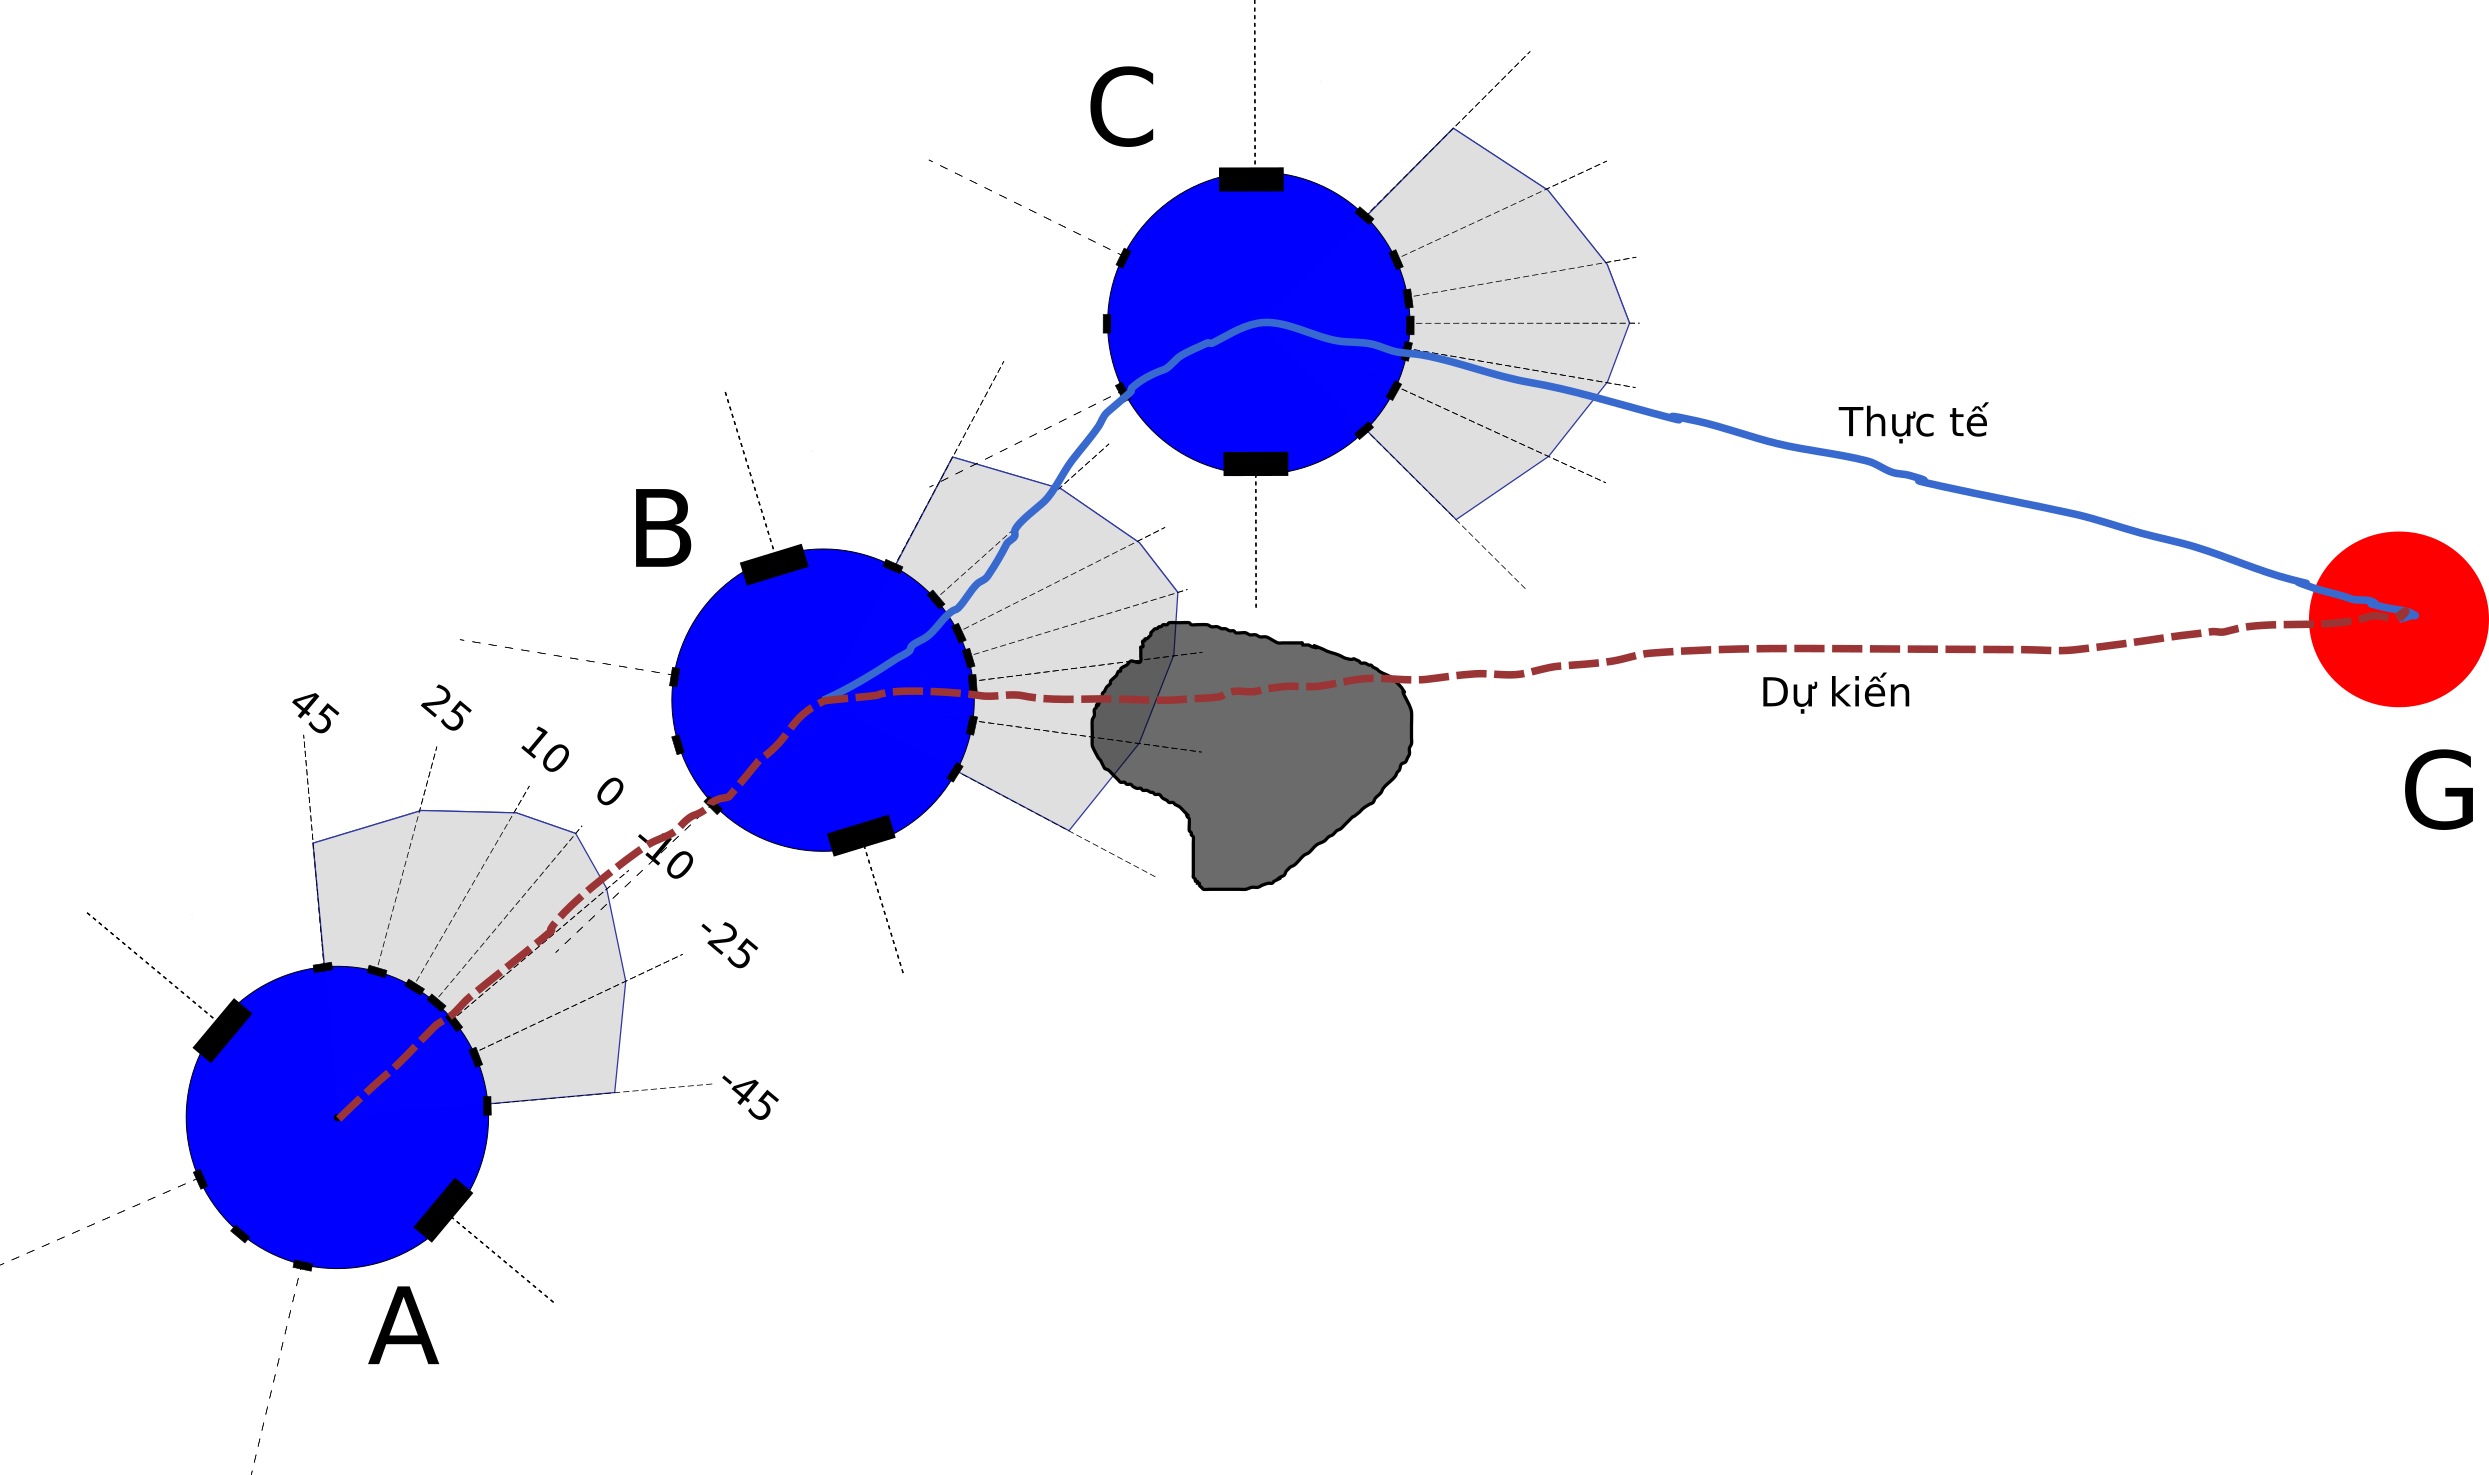
\includegraphics[width=0.75\linewidth]{figures/IR_BB-avoidance.png}} \\
    \subfloat[]{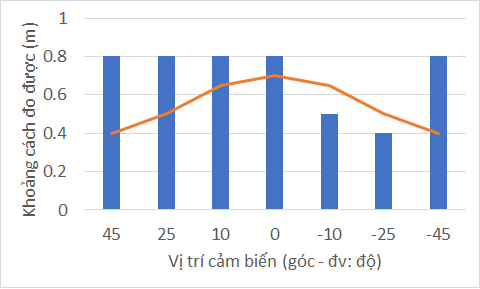
\includegraphics[width=0.5\linewidth]{figures/BB_chart.png}}
    \caption{Giải thuật tránh vật cản bằng bong bóng phản ứng}
    \label{fig:BB-avoidance}
\end{figure}

\textbf{Bong bóng phản ứng B}:
Trên cơ sở tham khảo \cite{Susnea2009}, thuật toán bong bóng phản ứng xác định một đường bao phía trước robot, có hình dạng như trong Hình \ref{fig:BB-argorithm}, kích thước đường bao được làm mới sau mỗi chu kì ${\Delta}{t}$, phụ thuộc vào vị trí cảm biến và vận tốc di chuyển của robot theo công thức \ref{equa:BB-update}. Trong đó $bb[i]$ là kích thước bong bóng tại vị trí cảm biến thứ i, $K_i$ là hệ số, $V_t$ là vận tốc dài của robot tại thời điểm t, $\Delta_t$ là khoảng thời gian giữa 2 lần cập nhật.
Kích thước đường bao là phạm vi đảm bảo robot có thể di chuyển tự do trong khoảng thời gian $\Delta_t$ mà không va chạm với vật cản.

\begin{equation}
    bb[i] = K_i*V_t*\Delta_t
    \label{equa:BB-update}
\end{equation}

\figurename{ \ref{fig:BB-avoidance}}a mô tả robot di chuyển từ vị trí A tới đích G với quỹ đạo được tính toán dự kiến theo đường nét đứt. Tuy nhiên, trên quá trình di chuyển, đến vị trí B, robot phát hiện thấy vật cản. Giá trị đo được của cảm biến và giá trị bong bóng phản ứng tại điểm B được mô tả trong biểu đồ Hình \ref{fig:BB-avoidance}b.
% trí gặp vật cản robot thực hiện quay mình để tránh vật cản, sau đó phần điều hướng trong robot lại tính lại đường đi tới đích (đường màu xanh).

\subsection{Phối hợp phân mức điều khiển}
Robot có nhiều chương trình khác nhau có thể tác động đến việc di chuyển của nó. Ví dụ trong phần lớn thời gian robot di chuyển dưới sự điều khiển của chương trình \codeword{navigation}, khi cần điều khiển bằng tay, robot lại chạy dưới sự điều khiển của chương trình \codeword{teleop}, khi gặp vật cản được phát hiện bởi cảm biến sonar, robot phản ứng lại. Như trường hợp đơn giản vừa rồi có tới ba tiến trình cùng đồng thời điều khiển robot.

\begin{figure}[htbp]
    \centering
    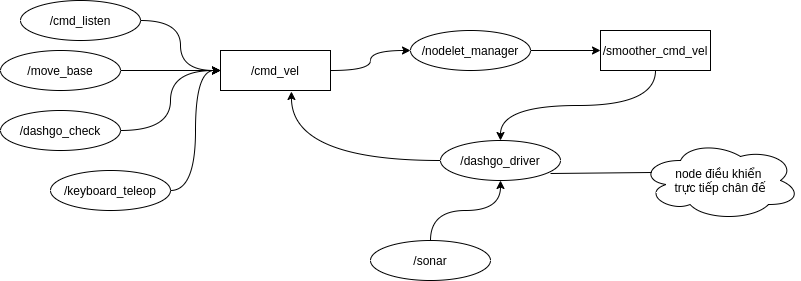
\includegraphics[width=\linewidth]{figures/phanquyen-goc.png}
    \caption{Các topic điều khiển robot}
    \label{fig:phanquyen-goc}
\end{figure}

\figurename{ \ref{fig:phanquyen-goc}} thể hiện các node và topic điều khiển robot Dashgo D1. Trong đó, topic \codeword{/cmd_vel} nhận thông tin điều khiển di chuyển chân đế từ nhiều topic khác nhau. Sau đó thông qua trình quản lý \codeword{nodelet_manager} để chạy chương trình làm mịn tốc độ, chống giật cho robot. \codeword{/smoother_cmd_vel} được topic \codeword{/dashgo_driver} nhận và thực hiện các tính toán điều khiển tới vòng quay của động cơ để di chuyển.
Ta thấy có \codeword{/sonar} được liên kết trực tiếp với \codeword{/dashgo_driver}, ở robot này, dữ liệu từ các cảm biến siêu âm được driver điều khiển chân đế đọc trực tiếp, sau đó xử lý các tình huống và tính toán số vòng quay của động cơ để thực hiện điều khiển chân đế trong trường hợp khẩn cấp.

% \subsection{Phương pháp phối hợp phân mức điều khiển}

\begin{figure}[htbp]
    \centering
    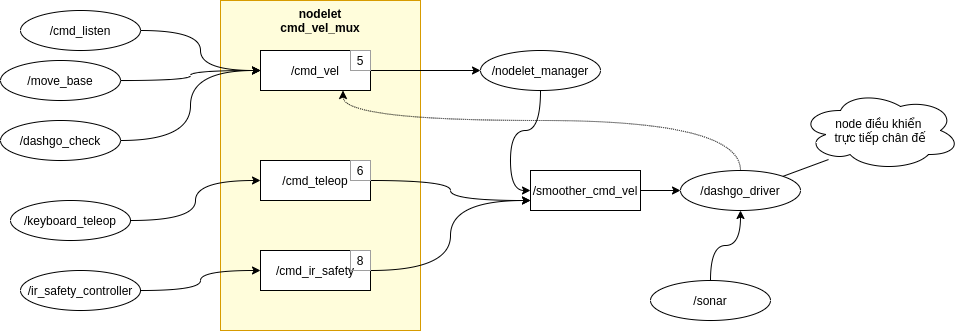
\includegraphics[width=\linewidth]{figures/phanquen-dexuat.png}
    \caption{Thiết kế phân quyền điều khiển}
    \label{fig:phanquen-dexuat}
\end{figure}

Có một vài phương pháp để phối hợp phân quyền điều khiển cho robot. Khi chúng ta có nhiều thuật toán, nhiều chương trình cùng điều khiển tới một hoạt động nào đó.
% ROS có định nghĩa \codeword{nodelet}\footnote{\url{http://wiki.ros.org/nodelet}}.
Trong luận văn này, tác giả sử dụng \codeword{cmd_vel_mux} của \codeword{nodelet} để thực hiện phân quyền điều khiển cho robot để dễ dàng tích hợp tín hiệu điều khiển từ cảm biến an toàn IR (Hình \ref{fig:phanquen-dexuat})

%=======================================
% \section{Đánh giá hệ thống tránh vật cản}}
\section{Kết quả và đánh giá}
\label{sec:testbed}

%---
% - Tiến hành thí nghiệm, nêu rõ bài toán thí nghiệm
% - Đánh giá kết quả (Hiệu quả hay không, vì sao)
%---

\subsection{Kết quả của luận văn}

Sau quá trình nghiên cứu và làm việc, tác giả đã có một số kết quả như sau:
\begin{itemize}
    \item Làm chủ hệ thống điều khiển robot, tạo bản đồ và di chuyển trong bản đồ.
    \item Phát triển hệ thống phần cứng robot. Hình \ref{fig:RB-multi-sensor-layer} là kết quả sau khi lắp hệ thống lên robot, robot có thể phát hiện và tránh vật cản bằng 3 tầng cảm biến siêu âm, lidar và hồng ngoại.
    \item Đề xuất và thử nghiệm hệ thống tránh vật cản bằng cảm biến đa tầng, bao gồm bố trí cảm biến, xử lý tín hiệu đo, giải thuật điều khiển.
    \item Nghiên cứu xây dựng hệ thống điều khiển phân quyền nhiều mức ưu tiên cho robot.
\end{itemize}

\begin{figure}[htbp]
    \centering
    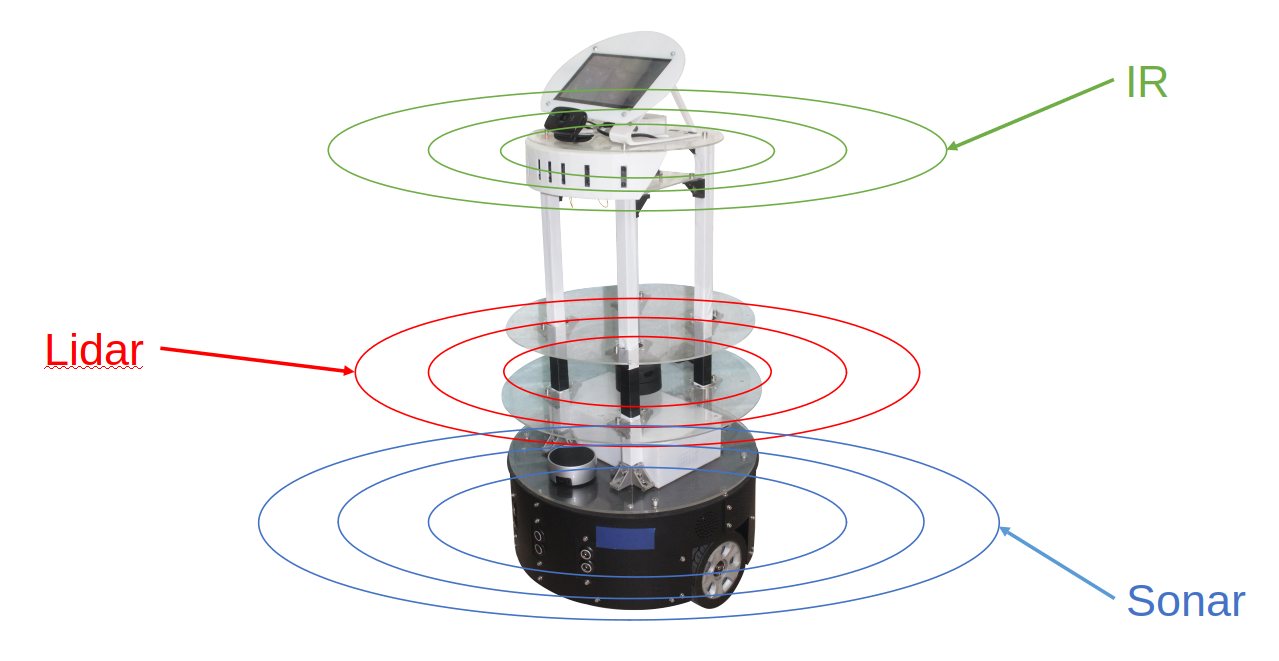
\includegraphics[width=0.75\linewidth]{figures/rb_Multi_Sensor_layer.png}
    \caption{Ba tầng cảm biến phát hiện vật cản trên robot}
    \label{fig:RB-multi-sensor-layer}
\end{figure}

\subsection{Đánh giá độ chính xác cảm biến khoảng cách hồng ngoại}
\label{sub:DanhgiaCBIR}
%------------------------------------------

Thực hiện đánh giá độ chính xác của cảm biến khoảng cách hồng ngoại IR Sharp GP2Y0A21YK0F. Tác giả bố trí thí nghiệm đo trên từng cảm biến riêng lẻ. Kết quả đo tại 8 vị trí khoảng cách 0.1m, 0.2m, 0.3m, 0.4m, 0.5m, 0.6m, 0.7m, 0.8m với 100 lần lấy mẫu, tần số lấy mẫu là 20Hz được kết quả đo như biểu đồ Hình \ref{fig:Ir-eval-100}.

\begin{figure}[htbp]
    \centering
    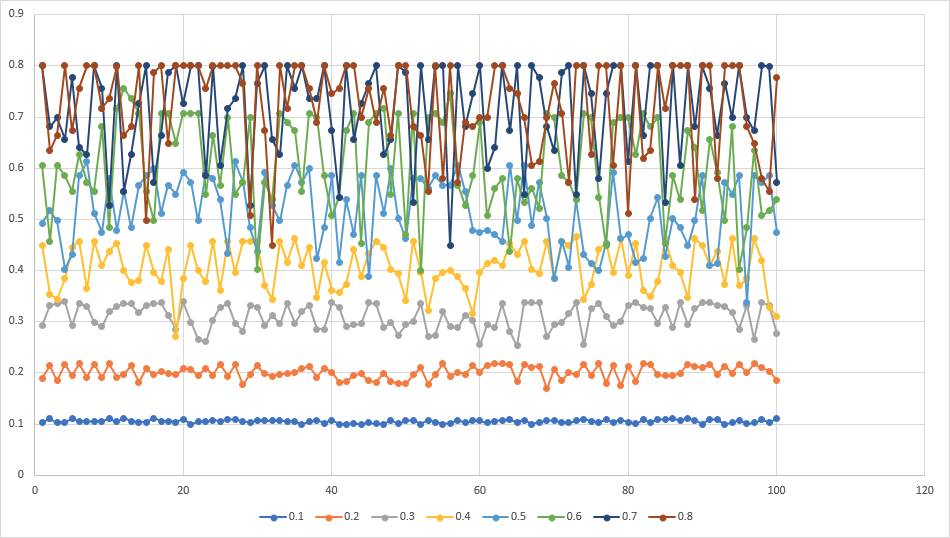
\includegraphics[width=\linewidth]{figures/IR-eval-chart.png}
    \caption{Kết quả đo cảm biến}
    \label{fig:Ir-eval-100}
\end{figure}

\begin{table}[htbp]
    \begin{tabular}{|m{1.5cm}|m{1.2cm}|m{1.2cm}|m{1.2cm}|m{1.2cm}|m{1.2cm}|m{1.2cm}|m{1.2cm}|m{1.4cm}|}
        \hline
        Cần đo     & 0.1      & 0.2      & 0.3      & 0.4      & 0.5      & 0.6      & 0.7      & 0.8      \\ \hline
        Trung bình & 0.1051   & 0.2009   & 0.3100   & 0.4068   & 0.5157   & 0.6086   & 0.7146       & 0.7229 \\ \hline
        Sai số & 0.0051 & 0.0009 &   0.0100 & 0.0068 &   0.0157 & 0.0086 &   0.0146 & -0.0771 \\ \hline
        \% sai số  & 5.14\% & 	0.44\% &	3.34\% &	1.69\% &	3.14\% &	1.43\% &	2.08\% &	9.63\% \\
        \hline
    \end{tabular}
    \caption{Giá trị đo trung bình 100 mẫu}
    \label{table:ir-evarage}
\end{table}


\begin{figure}[htbp]
    \centering
    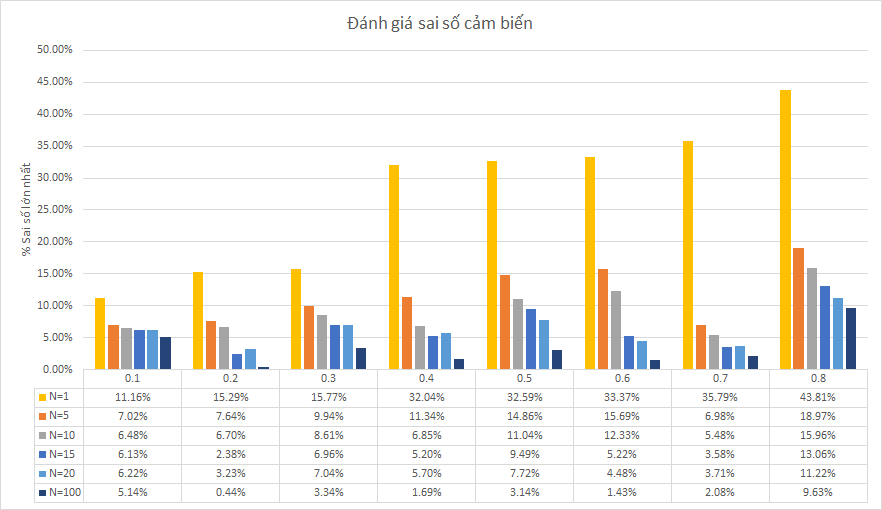
\includegraphics[width=\textwidth]{figures/chart_IReval_MaxPercent.png}
    \caption[Đánh giá sai số lớn nhất tương ứng với số lần lấy mẫu]{Đánh giá sai số lớn nhất tương ứng với số lần lấy mẫu trên một lần đo N = 1, 5, 10, 15, 20 và 100}
    \label{chart:IR-eval-NumSample}
\end{figure}

 Giá trị trung bình của 100 lần đo và sai số được thể hiện trong Bảng \ref{table:ir-evarage}. Từ đây ta thấy với trung bình của 100 lần đo thì sai số nằm trong giới hạn sai số cho phép 5\% với phép đo trong khoảng 0.1-0.7m.
%  Do cảm biến IR Sharp GP2Y0A21YK0F có khoảng đo từ 10 - 80 cm nên tác giả đã đặt khoảng cách đo giới hạn từ 10 - 80 cm. Do đó trong biểu đồ Hình \ref{fig:Ir-eval-100} kết quả đo bị chặn dưới tại 0.1m và chặn trên tại 0.8m.
%  Hình \ref{fig:IR-evel-N1} thể hiện sai số trong phép đo cảm biến.

\begin{figure}[htbp]
\centering
\subfloat[][]{
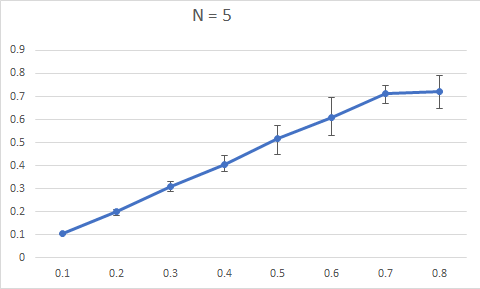
\includegraphics[width = 0.45 \linewidth]{figures/chart_IReval_N5.png}
}
\subfloat[][]{
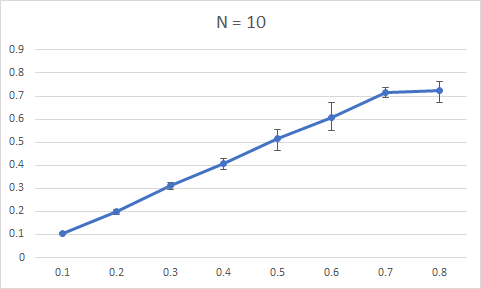
\includegraphics[width = 0.45 \linewidth]{figures/chart_IReval_N10.png}
}
\hspace{8pt}
\subfloat[][]{
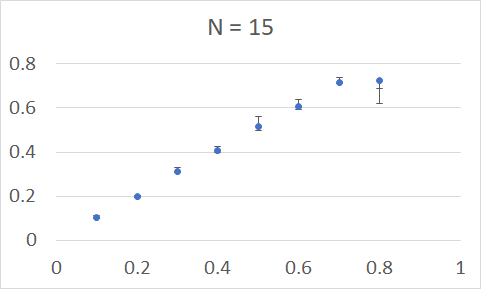
\includegraphics[width = 0.45 \linewidth]{figures/chart_IReval_N15.png}
}
\subfloat[][]{
    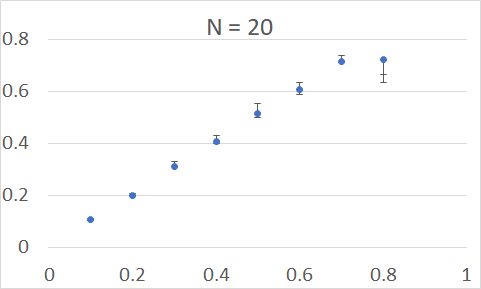
\includegraphics[width = 0.45 \linewidth]{figures/chart_IReval_N20.png}
    }
    \caption{Sai số tương ứng với N lần lấy mẫu}
    \label{fig:chart-IR-N-errorbar}
\end{figure}

Tác giả áp dụng bộ lọc trung bình cộng (công thức \ref{equa:Med_filter}) để giảm nhiễu và sai số trong kết quả đo. Tuy nhiên, trong thực tế, robot di chuyển theo thời gian thực, do đó số lần lấy mẫu cho một lần đo N bị giới hạn. Biểu đồ Hình \ref{chart:IR-eval-NumSample} đánh giá sai số lớn nhất với các giá trị N khác nhau. Hình \ref{fig:chart-IR-N-errorbar} thể hiện mức độ hội tụ của kết quả đo tương ứng với các giá trị N khác nhau. Qua đây chúng ta có thể thấy khi tăng N thì sai số trong phép đo càng giảm và giá trị đo càng hội tụ. Tuy nhiên, để đảm bảo robot cập nhật kết quả đo theo thời gian thực, tác giả chọn N = 10 tương ứng với tần số cập nhật kết quả đo là 2 lần/giây.

%============================================================
\subsection{Đánh giá giải thuật điều khiển tích hợp cảm biến}
%------------------------------------------------------------
% \subsubsection*{Phương pháp đánh giá}
% \subsubsection*{Kết quả đạt được}


Ưu điểm của hệ thống tránh vật cản bằng phối hợp nhiều tầng cảm biến là robot có thể di chuyển an toàn được trong các môi trường với đa dạng đối tượng hơn như bàn, ghế, các đối tượng mà bài toán định vị dẫn đường 2D chỉ với một tầng cảm biến có thể không đáp ứng được khi vật cản không nằm trong mặt phẳng quét của LIDAR.

\begin{figure}[htbp]
    \centering
    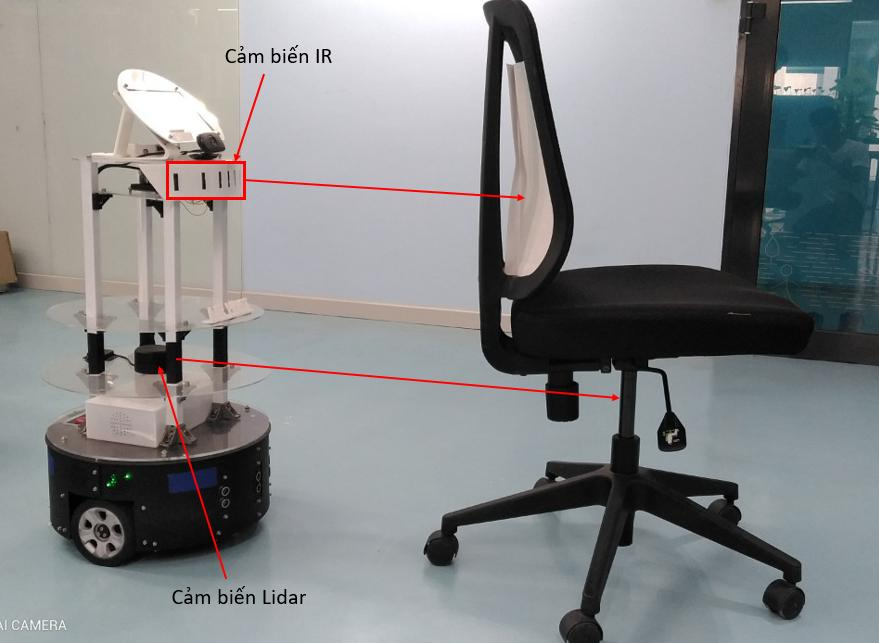
\includegraphics[width=0.5\linewidth]{figures/RB_scenario_ir_detectingObstacle.png}
    \caption{Robot với vật cản có biên dạng biến đổi theo chiều cao}
    \label{fig:scenario_ir_detectedObstacle}
\end{figure}

\begin{figure}[htbp]
    \centering
    \subfloat[]{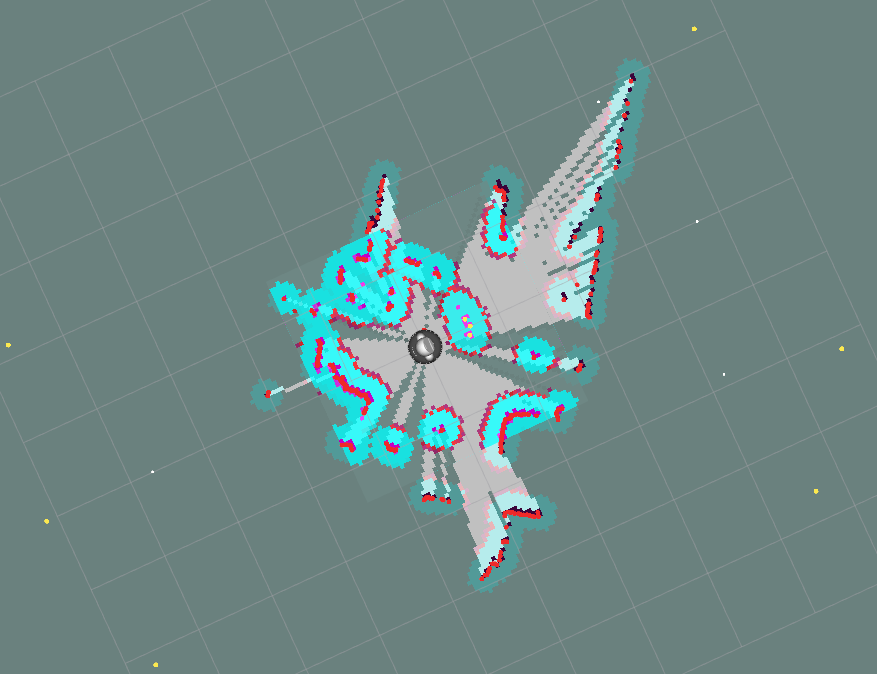
\includegraphics[width=0.75\linewidth]{figures/RB_withIR_ObstacleDetected.png}}
    \hspace{8pt}
    \subfloat[]{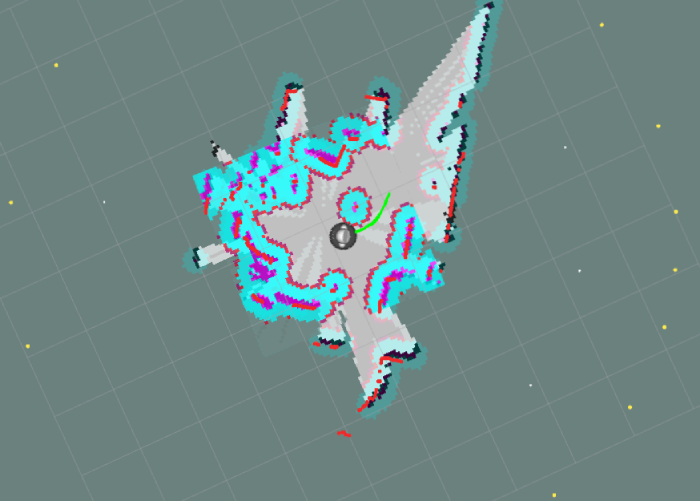
\includegraphics[width=0.75\linewidth]{figures/RB_withIR_navigation.png}}
    \caption{Hệ thống cảm biến hồng ngoại phát hiện vật cản và đánh dấu vào bản đồ giá trị (costmap)}
    \label{fig:rb_withIR_ObstacleDetected}
\end{figure}

\begin{figure}[htbp]
    \centering
    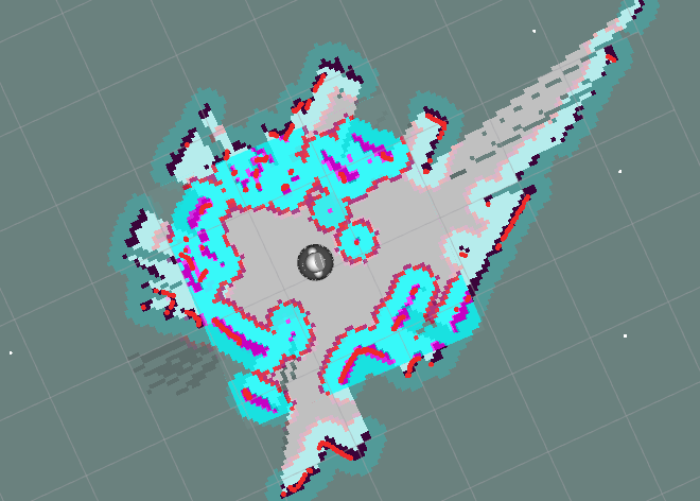
\includegraphics[width=0.75\linewidth]{figures/RB_withoutIR_obstacleDetect.png}
    \caption{Trường hợp không kích hoạt lớp tránh vật cản bằng hồng ngoại}
    \label{fig:rb_withoutIR}
\end{figure}

Tác giả đã phát triển hệ thống cảm biến hồng ngoại, phát hiện và tránh được vật cản. Đồng thời phối hợp với hai tầng cảm biến sẵn có trên robot là cảm biến LIDAR và cảm biến tránh vật cản bằng siêu âm. Khi xuất hiện vật cản, robot sẽ tránh theo giải thuật được mô tả tại mục \ref{sec:caitienhethongtranhvatcan} và đồng thời đánh dấu vật cản vào bản đồ cục bộ để giúp robot tạo đường đi mới mà không lặp lại đường cũ.

Hình \ref{fig:scenario_ir_detectedObstacle} thể hiện một trường hợp mà robot đối diện với vật cản có hình dạng biến đối theo chiều cao. Với hệ thống tránh vật cản chỉ có lidar, robot chỉ có thể phát hiện được phần thân dưới rất bé của đối tượng như Hình \ref{fig:rb_withoutIR} chỉ phát hiện thấy một chấm tròn. Tuy nhiên, với hệ thống mới mà tác giả đề xuất, robot có thể phát hiện được phần biên dạng phía trên của đối tượng và đánh dấu là vật cản trong bản đồ Hình \ref{fig:rb_withIR_ObstacleDetected}. Do đó, khi cho robot di chuyển tới vị trí phía sau đối tượng, robot tạo đường đi tránh vật cản và di chuyển vòng qua nó như trong Hình \ref{fig:rb_withIR_ObstacleDetected}b.

Tuy nhiên, hệ thống còn có một số điểm hạn chế như:
\begin{itemize}
    \item Hệ thống cảm biến đo chưa thực sự chính xác và ổn định, gây ra khó khăn trong quá trình áp dụng thuật toán
    \item Cảm biến hồng ngoại IR Sharp GP2Y0A21YK0F có tần số lấy mẫu tương đối thấp (tối đa 26Hz), do đó không thể tăng số lần lấy mẫu trong một lần đo, gây ảnh hưởng tới độ chính xác của kết quả đo. Bên cạnh đó, cảm biến này có khoảng đo từ 0.1-0.8m do vậy robot chỉ có thể phát hiện được vật cản trong khoảng này, điều này làm hạn chế tốc độ di chuyển có thể tránh được vật cản của robot.
\end{itemize}

% \begin{itemize}
%     \item Đánh giá cảm quan robot di chuyển và tránh được vật cản trong quá trình di chuyển ở tầng cảm biến hồng ngoại
%     \item Thực hiện thí nghiệm cho robot di chuyển giữa các điểm bất kì trong một môi trường đã được xây dựng bản đồ với các vật có hình dạng đa dạng từ thấp tới cao. Đánh giá về số lần tránh được/không tránh được vật cản
% \end{itemize}

%TODO: Bổ sung kq đánh giá thí nghiệm di chuyển

%=============================
\chapter{Kết luận và tầm nhìn}
\label{chap:KetLuan}

\section{Kết luận}
                %------------------
% Tóm tắt lại luận văn

Như vậy, trong luận văn này, tác giả đã đề cập tới các vấn đề, bài toán trong robot tự hành và một số đóng góp của tác giả với một số kết quả chính như sau:
\begin{itemize}
    \item Giới thiệu Robot tự hành, ứng dụng và các bài toán
    \item Đề xuất phương pháp nâng cao độ an toàn trong di chuyển của robot bằng cách thêm một tầng cảm biến khoảng cách hồng ngoại. Tham khảo và đề xuất giải thuật điều khiển robot với nhiều tầng cảm biến.
    \item Thực hiện thí nghiệm và đánh giá hiệu quả mà phương pháp mang lại.
\end{itemize}


\section{Tầm nhìn}
% Hướng nghiên cứu tiếp theo
% Tối ưu hệ thống hiện tại
%------------------------
Trên Thế giới, robot tự hành thông minh đã được ứng dụng trong nhiều lĩnh vực khác nhau như đã đề cập ở \ref{sec:ungdung}. Tuy nhiên, ở Việt Nam chúng ta ứng dụng của robot tự hành thông minh rất ít, chủ yếu trong công nghiệp, hỗ trợ vận chuyển trong các nhà máy, kho hàng. Với các yêu cầu khắt khe khi đi vào thực tế. Trong thời gian tới, có một số hướng để phát triển robot tự hành thông minh như sau:
\begin{itemize}
    \item Tối ưu và tăng tính ổn định, tin cậy cho giải thuật tránh vật cản.
    \item Xây dựng chương trình để vận hành robot một cách đơn giản, hiệu quả và ổn định.
    \item Nghiên cứu và ứng dụng một số kết quả mới trong bài toán định vị và dẫn đường trong robot.
    \item Ứng dụng một số bài toán mới như xử lý ảnh ứng dụng học sâu, xử lý tiếng nói, chatbot\dots vào điều khiển robot.
\end{itemize}



%%%=======================
%%% Local Variables:
%%% mode: latex
%%% TeX-master: "../LuanVanThS_v1.0_main"
%%% End:
